\chapter{Anforderungsanalyse}
\label{sec:requirements}
% Wie ist die Ausgangslage (in Bamberg)? Wie werden/wurden die Anforderungen aufgestellt, 
% wer sind die Stakeholder und warum? Dann Anforderungen definieren und priorisieren
Bevor mit der eigentlichen Implementierung begonnen werden kann, ist es notwendig, die Anforderungsanalyse. Der erste Schritt hierzu besteht daraus, die Ausgangslage in Bamberg zu untersuchen, um darauf aufbauend die Stakeholder zu identifizieren, da diese den Ursprung der Anforderungen darstellen. Nachdem das Aufstellen der Anforderungen erfolgreich gewesen ist, können diese im Anschluss analysiert, also priorisiert, auf ihre Validität und im Anschluss auf ihre Realisierbarkeit überprüft werden. Basierend auf den Anforderungen werden dann Use Cases formuliert, die die Anforderungen in einer konkreten Situation beschreiben und damit die Grundlage für die Implementierung bilden.

\section{Ausgangslage in Bamberg}
\label{sec:ausgangslage}
Bamberg\sidenote{\url{https://www.stadt.bamberg.de/Unsere-Stadt/Stadtinfo/}} ist eine kreisfreie Stadt in Bayern im Regierungsbezirk Oberfranken mit einer Einwohnerzahl von knapp 80.000 Einwohnern (Stand: Dezember 2022). Die Stadt selbst kann dabei in sogenannte \ac{LCZ}, also Klassifikationen, welche sich durch die logische Aufteilung einer Landschaft ergeben \cite{stewart2011local}, unterteilt werden. Zusammen mit dem Domänenwissen des Meteorologen Prof.\ Dr.\ Thomas Foken (vgl. Kapitel \ref{sec:stakeholder}) hat eine rudimentäre Unterteilung in sechs \ac{LCZ} stattgefunden: Die Innenstadt, die ERBA, Gartenstadt, Bamberg-Ost, der Hain, am Laubanger und das Berggebiet (siehe Abbildung \ref{fig:lcz}). Die Entscheidung über die Grenzen und der Gebiete erfolgt dabei durch die in der Literatur gegebenen Charakteristika, welche zum Definieren von \ac{LCZ} notwendig sind \cite{oke2004initial, stewart2012local}:

\keyword{Innenstadt (2)} -- Die Innenstadt kann als \enquote{Compact midrise} klassifiziert werden. Charakteristisch für diese \ac{LCZ} ist der dichte Mix aus mittelhohen Gebäuden, das Vorhandensein von wenigen bis keinen Bäumen und hauptsächlich asphaltierten Landflächen. Überwiegend lassen sich Stein, Ziegel, Kacheln und Beton als Baumaterialien vorfinden.

\keyword{ERBA (6)} -- Die ERBA kann als \enquote{Open low-rise} klassifiziert werden. In einem solchen befinden sich in der Regel flache Gebäude, die in einer offeneren Struktur angeordnet sind. Die Landflächen sind asphaltiert, weisen aber auch Grünflächen in Form von kleinen Pflanzen oder verstreuten Bäumen auf. Die Baumaterialien sind ähnlich wie in der Innenstadt, jedoch kann man an der ERBA häufig Holz als Baumaterial vorfinden.

\keyword{Gartenstadt (6B)} -- Die Gartenstadt ist wie die ERBA ein \enquote{Open low-rise}. Allerdings kann hier der Zusatz \textit{\enquote{B}} als \enquote{Land cover type}\sidenote{Nach \cite{stewart2012local}: Klassifikationen zu saisonalen Eigenschaften, wie z.B. schneebedeckter Boden, trockener/feuchter Boden etc.} zur Klassifikation hinzugefügt werden, welche nach \cite{stewart2012local} bedeutet, dass die Landschaft rege mit immergrünen Bäumen bestückt ist. Die Landflächen weisen zu einem Großteil Grünflächen mit kleinen Pflanzen auf. Diese Arten von \ac{LCZ} werden in der Regel für Wälder oder Stadtparks verwendet.

\keyword{Bamberg-Ost (3)} -- Der Osten Bambergs wird als \enquote{Compact low-rise} klassifiziert. Dieser weist die identischen Charakteristika wie die Bamberger Innenstadt auf, mit dem einzigen Unterschied, dass es sich bei den Gebäuden um niedrige Gebäude handelt.

\keyword{Hain (5)} -- Der Hain befindet sich in der Klasse des \enquote{Open midrise}. Dieser weist die identischen Charakteristika wie die ERBA auf, mit dem einzigen Unterschied, dass es sich bei den Gebäuden um mittelhohe Gebäude handelt und statt Holz überwiegend Beton und Stahl als Baumaterialien eingesetzt werden.

\keyword{Laubanger (8)} -- Der Laubanger wird in Bamberg als \enquote{Large low-rise} eingestuft. In dieser Klasse lassen sich in der Regel große, aber flache Gebäude in einer offeneren Struktur vorfinden. Bäume oder Grünflächen sind meistens nicht bis kaum vorhanden, da die Straßen und Wege überwiegend asphaltiert sind. Als Baumaterialien kommen häufig Stahl, Beton und Stein zum Einsatz.

\keyword{Berggebiet (6A)} -- Das Bamberger Berggebiet ähnlich wie die Gartenstadt und ERBA als \enquote{Open low-rise} eingestuft und weist die identischen Charakteristika auf. Der Zusatz \textit{\enquote{A}} besagt hierbei, dass eine große bzw. dichte Menge an Bäumen in der Landschaft vorzufinden ist, was in der Regel auch für Wälder oder Stadtparks zutrifft.

\begin{figure}[t] % [t]: place at top of page (recommended)
    \centering
    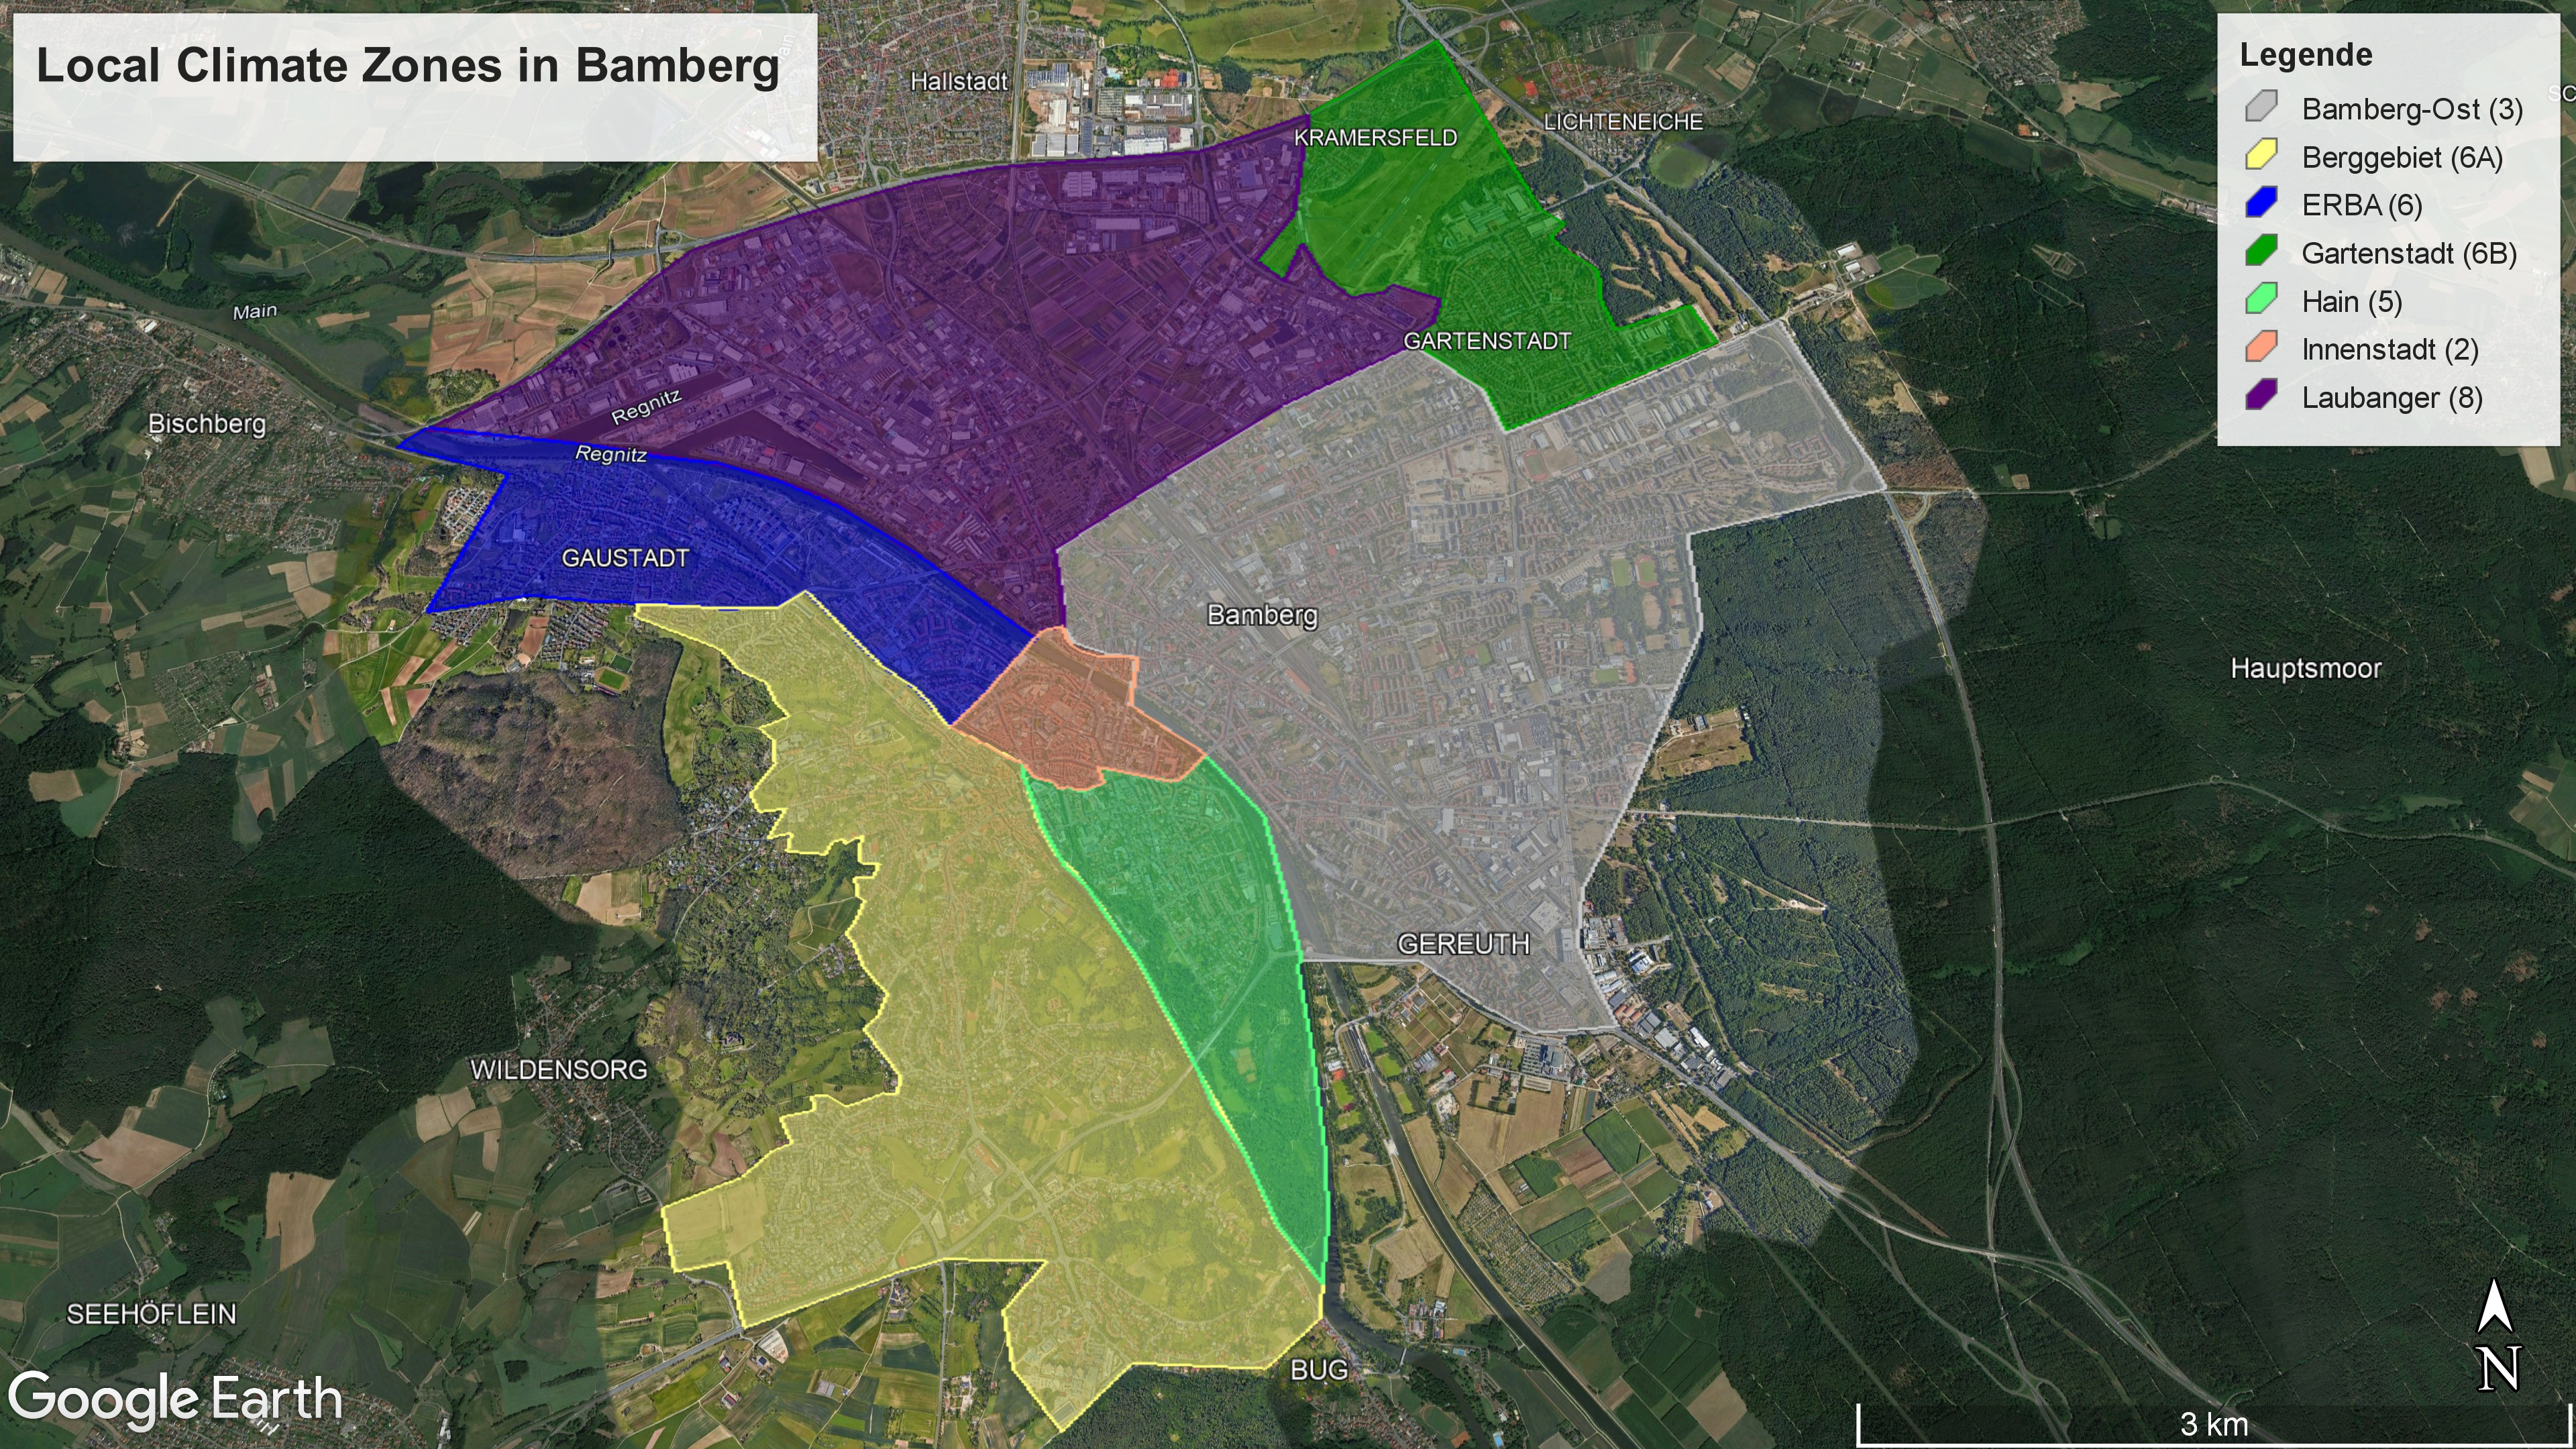
\includegraphics[width=1\textwidth]{figures/lcz.jpg}
    \decoRule
    \caption[LCZ in Bamberg]{Die sechs \ac{LCZ} in Bamberg (eigene Darstellung, basierend auf \cite{stewart2012local,oke2004initial})} 
    \label{fig:lcz}
\end{figure}

Durch die Unterteilung der Stadt Bamberg in \ac{LCZ} ist es möglich, die Auslesungen der Wetterstationen und die Unterschiede der Messwerte in den einzelnen Gebieten nachvollziehen und damit besser analysieren zu können. \\ In der Stadt selbst sind Wetterstationen\sidenote{Die genaue Anzahl der Sensoren ist unbekannt, da nicht alle öffentlich einsehbar sind (Stand Oktober 2023: 42 Wetterstationen einsehbar} verteilt, die jeweils die Temperatur und Luftfeuchtigkeit am entsprechenden Standort messen. Auf der Wetterkarte von Netatmo\sidenote{\url{https://weathermap.netatmo.com/}} sind diese Auslesungen von öffentlichen Netatmo-Wetterstationen einsehbar.

\subsection{Identifikation der Stakeholder}
\label{sec:stakeholder}
In diesem Abschnitt der Arbeit werden die Stakeholder identifiziert, dessen Bedürfnisse und Ansprüche durch die Entwicklung des interaktiven Werkzeuges befriedigt werden sollen. Diese werden im Folgenden vorgestellt:

\paragraph{Der Bürgerverein Bamberg Mitte e.V.}
Bei dem \ac{BVM} handelt es sich um einen Bürgerverein in der Stadt Bamberg, welcher 1905 gegründet wurde und mit zahlreichen Projekten\sidenote{\url{https://bvm-bamberg.de/de/projektseiten/projekte-und-aktivitaeten/}} und durch das Praktizieren von Bürgerbeteiligung die Stadt Bamberg, vor allem in Hinblick auf die Stadtplanung und des Umwelt- und Denkmalschutzes, mitgestaltet\sidenote{\url{https://bvm-bamberg.de/de/buergerverein/unser-verein/}}.

Eines dieser Projekte ist das \enquote{Klimamessnetz auf der Bamberger Inselstadt}. Hier wird seit Anfang 2022 mithilfe von insgesamt neun smarten Netatmo-Wetterstationen\sidenote{\url{https://shop.netatmo.com/de-de/weather/smart-weather-station/weatherstation}} (Stand: 21. Oktober 2023) ein Klimamessnetz im Bamberger Zentrum zum Messen der Temperatur und Luftfeuchtigkeit an den entsprechenden Standorten\sidenote{Standorte der smarten Wetterstationen (\ac{LCZ}): Steinertstraße (Innenstadt), Lange Straße (Innenstadt), Am Weidenufer (ERBA), Holzmarkt (Innenstadt), Promenadestraße (Innenstadt), Wetzelstraße (ERBA), Fischerei (Innenstadt), Frauenstraße (Innenstadt) und Hainstraße (Hain)} aufgebaut. \\ Aus den Messungen der Wetterstationen ergibt sich, dass sich die Bamberger Innenstadt im Vergleich zu anderen \ac{LCZ} kaum abkühlt und die Temperaturen sich häufig von der offiziellen Station des \ac{DWD} unterscheiden (vgl. Webauftritt\sidenote{\url{https://bvm-bamberg.de/de/projektseiten/klima/}} des \ac{BVM}). Dies ist auch darauf zurückzuführen, dass das Fehlen von Bäumen und Grünflächen als Charakteristika eines \enquote{Compact mid-rise} ausschlaggebend für das Aufwärmen der Innenstadt ist: Ein Team von Geoökologen der Universität ETH Zürich hat in einer Studie gezeigt, dass Grünanlagen mit Bäumen in Städten zu einem Kühlungseffekt führen \cite{bastin2019global}. Dieser Effekt entsteht durch die Tatsache, dass Bäume durch ihre Wurzeln mehr Wasser aufnehmen können, welches im Umkehrschluss an trockenen und heißen Tagen verdunsten und so zu einer Abkühlung führen kann \cite{bastin2019global}. \\ Wie in Kapitel \ref{sec:methodologyrequirements} bereits erläutert, trifft sich der \ac{BVM} in regelmäßigen Abständen zum Analysieren der Auslesungen der Wetterstationen und Diskutieren von Maßnahmen, die zur Abkühlung der Innenstadt beitragen können. Durch die Teilnahme an diesen Treffen und die daraus resultierenden Gespräche mit den Mitgliedern des \ac{BVM} wurde in Erfahrung gebracht, dass das grundlegende Ziel des Vereins ist, Führungspersonen (z.B. in der Politik, Stadtplanung, Ämtern etc.) durch die Auslesungen der Wetterstationen zu sensibilisieren und damit zu einer Verbesserung der Lebensqualität durch das Erreichen des Kühlungseffektes in der Stadt Bamberg beizutragen. Dies soll ihrer Ansicht nach durch das Reduzieren von Parkplätzen (zum Minimieren von stehen gelassenen Autos) und Straßen für Autos erreicht werden, sodass für die neu geschaffenen Flächen Bäume und Grünflächen gepflanzt werden können.

\paragraph{Die Domänenexpert*innen}
Als Domänenexpert*innen werden in dieser Arbeit Personen definiert, die durch ihre Expertise und Erfahrung in einer Domäne wichtige Einblicke und Informationen, die über die Literatur hinausgehen, zu einem Projekt beitragen können. Sowohl für dieses Projekt, als auch für das Projekt des \ac{BVM} fungiert hier Prof.\ Dr.\ Thomas Foken\sidenote{\url{https://www.micrometeorology.de/}}, der durch seine Professur für Mikrometeorologie an der Universität Bayreuth langjährige Erfahrung in der (Mikro-)Meteorologie und der Klimaforschung besitzt. Durch die Teilnahme Prof.\ Dr.\ Fokens an den regelmäßigen Treffen mit dem \ac{BVM} ist es möglich gewesen, Erläuterungen und Definition der (Mikro-)Meteorologie zu erhalten, sodass erste Fokusse der Arbeit gesetzt werden konnten: \\ Einer dieser Punkte sind die sogenannten \enquote{Tropennächte}\sidenote{Nächte, in denen die minimale Temperatur zwischen 18 und 6 Uhr UTC mindestens 20°C betragen hat \cite{TropennachtDWD}} in Deutschland gewesen, die den Analysen des Professors nach eine deutliche Steigung in den letzten Jahren aufweisen. Dieser Aspekt ist insofern gefährlich für den Menschen, da der Körper des Menschen durch eine solche Hitzebelastung auf eine besondere Weise beansprucht wird und Probleme, die sich auf das Herz-Kreislaufsystem des Menschen auswirken, auftreten können \cite{Umweltbundesamt2023Hitze}
Tropennächte bieten sich insofern als guter Messwert an, da diese Kennzeichen für Hitzewellen in relativ kühleren Regionen der Welt (\textit{hier:} Deutschland) und für ihre geringe Frequenz eigentlich eine Ausnahmeerscheinung repräsentieren sollten TODO HIER ZITAT. [...]

\paragraph{Der \ac{MOBI-Lehrstuhl}}
Der \ac{MOBI-Lehrstuhl}\sidenote{\url{https://www.uni-bamberg.de/mobi/}} ist ein Lehrstuhl, welcher 2014 in der Fakultät Wirtschaftsinformatik und Angewandte Informatik an der Otto-Friedrich-Universität Bamberg angelegt wurde. Die Leitung übernimmt Prof.\ Dr.\ Daniela Nicklas, welche gleichzeitig die Betreuerin dieser Arbeit darstellt. Der Lehrstuhl beschäftigt sich insbesondere mit den \enquote{Fragen des Datenmanagements für mobile Systeme, Datenstrommanagement/komplexe Ereignisverarbeitung und der Unterstützung sensorbasierter Anwendungen, unter anderem im Bereich Smart Cities}. Die Hauptansprechpartner*innen im Rahmen dieser Arbeit sind Prof.\ Dr.\ Daniela Nicklas, Leonie Ackermann und Aboubakr El Hacen Benabbas gewesen. \\ Der MOBI-Lehrstuhl hat ebenfalls an den regelmäßigen Treffen des \ac{BVM} zusammen mit Prof.\ Dr.\ Thomas Foken teilgenommen, sodass hier zusätzlich die Möglichkeit bestanden hat, Erfahrungen und Wissen aus dem Bereich der Informatik, der Datenverarbeitung und notwendige Schritte zum Entwickeln eines interaktiven Werkzeuges zu erhalten. Im gemeinsamen Austausch wurden Anforderungen ausgearbeitet, die sowohl für das \ac{BVM} und die Domänenexpert*innen in Hinblick auf die Auslesungen der Wetterstationen und die damit verbundenen Analysen der Sensordaten, als auch für den \ac{MOBI-Lehrstuhl} in Hinblick auf die technische Umsetzung relevant, aber auch realistisch sind. 

\paragraph{Weitere Stakeholder}
Da eine Stadt selbst nicht als Stakeholder identifiziert werden kann, weil eine solche keine eigene Entscheidungs- bzw. Handlungseinheit darstellt, sollte Bamberg selbst trotzdem in diesem Abschnitt erwähnt werden. Dies ist darauf zurückzuführen, dass im Idealfall die eingesetzte Software Regierungsbehörden, Verwaltungen oder ähnliche Organisationen der Stadt erreichen kann und im Idealfall die Auswirkungen dieser Sache Bürger*innen, Unternehmen oder andere Interessensgruppen innerhalb der Stadt betreffen. Allerdings hat zum Zeitpunkt der Anforderungsanalyse weder mit der Stadt Bamberg, noch mit den Bürger*innen ein Austausch stattgefunden, sodass diese als indirekter Stakeholder erwähnt, aber weiterführend in dieser Arbeit nicht betrachtet werden.

Die in diesem Kapitel erläuterten Stakeholder wurden zum Zeitpunkt der Anforderungsanalyse identifiziert. Eine Limitierung auf diese Stakeholder ist aber nicht gegeben, sodass im Laufe der Arbeit oder in der Zukunft weitere Stakeholder identifiziert und in die Anforderungsanalyse aufgenommen werden können.
% \subsection{Das Bamberger Klimamessnetz als Grundlage der Sensordaten}

\section{Die Netatmo API --- eine Schnittstelle zwischen Sensordaten und Stakeholder}

\section{Definition der Anforderungen}

\section{Use Cases}